\documentclass[a4paper,12pt]{article} 

% First, we usually want to set the margins of our document. For this we use the package geometry.
\usepackage[top = 2.5cm, bottom = 2.5cm, left = 2.5cm, right = 2.5cm]{geometry} 
\usepackage[T1]{fontenc}
\usepackage[utf8]{inputenc}

% The following two packages - multirow and booktabs - are needed to create nice looking tables.
\usepackage{multirow} % Multirow is for tables with multiple rows within one cell.
\usepackage{booktabs} % For even nicer tables.

% As we usually want to include some plots (.pdf files) we need a package for that.
\usepackage{graphicx} 

% The default setting of LaTeX is to indent new paragraphs. This is useful for articles. But not really nice for homework problem sets. The following command sets the indent to 0.
\usepackage{setspace}
\setlength{\parindent}{0in}

% Package to place figures where you want them.
\usepackage{float}

% The fancyhdr package let's us create nice headers.
\usepackage{fancyhdr}

\usepackage{amsmath,amsthm,caption}
\usepackage[open]{bookmark}
\usepackage{minted}
\usepackage{paracol}


% To make our document nice we want a header and number the pages in the footer.

\pagestyle{fancy} % With this command we can customize the header style.

\fancyhf{} % This makes sure we do not have other information in our header or footer.

\lhead{\footnotesize Operating System (H): Assignment 7}% \lhead puts text in the top left corner. \footnotesize sets our font to a smaller size.

%\rhead works just like \lhead (you can also use \chead)
\rhead{\footnotesize Mengxuan Wu} %<---- Fill in your lastnames.

% Similar commands work for the footer (\lfoot, \cfoot and \rfoot).
% We want to put our page number in the center.
\cfoot{\footnotesize \thepage} 

\begin{document}

\thispagestyle{empty} % This command disables the header on the first page. 

\begin{tabular}{p{15.5cm}}
{\large \bf Operating System (H)} \\
Southern University of Science and Technology \\ Mengxuan Wu \\ 12212006 \\
\hline
\\
\end{tabular}

\vspace*{0.3cm} %add some vertical space in between the line and our title.

\begin{center}
	{\Large \bf Assignment 7}
	\vspace{2mm}

	{\bf Mengxuan Wu}
		
\end{center}  

\vspace{0.4cm}

I choose the \texttt{lat\_pipe} test script to analyze. The result and flame graph are shown below.

\begin{figure}[H]
	\centering
	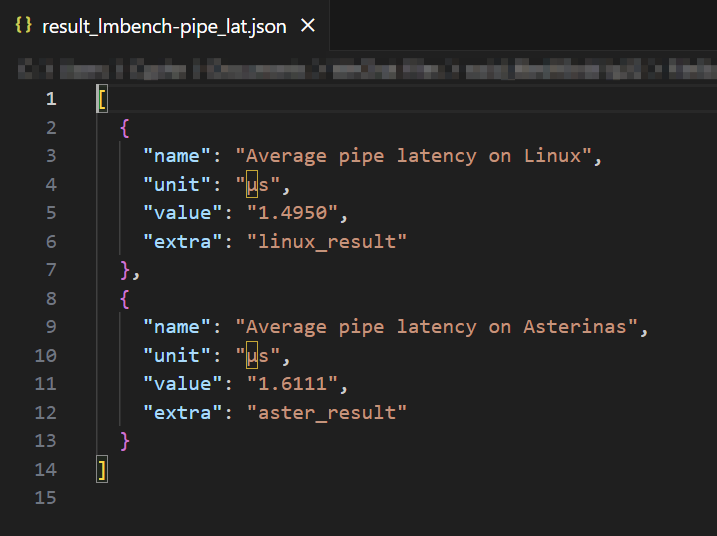
\includegraphics[width=0.8\textwidth]{figure/json_result.png}
	\caption{Result of \texttt{lat\_pipe}}
\end{figure}

\begin{figure}[H]
	\centering
	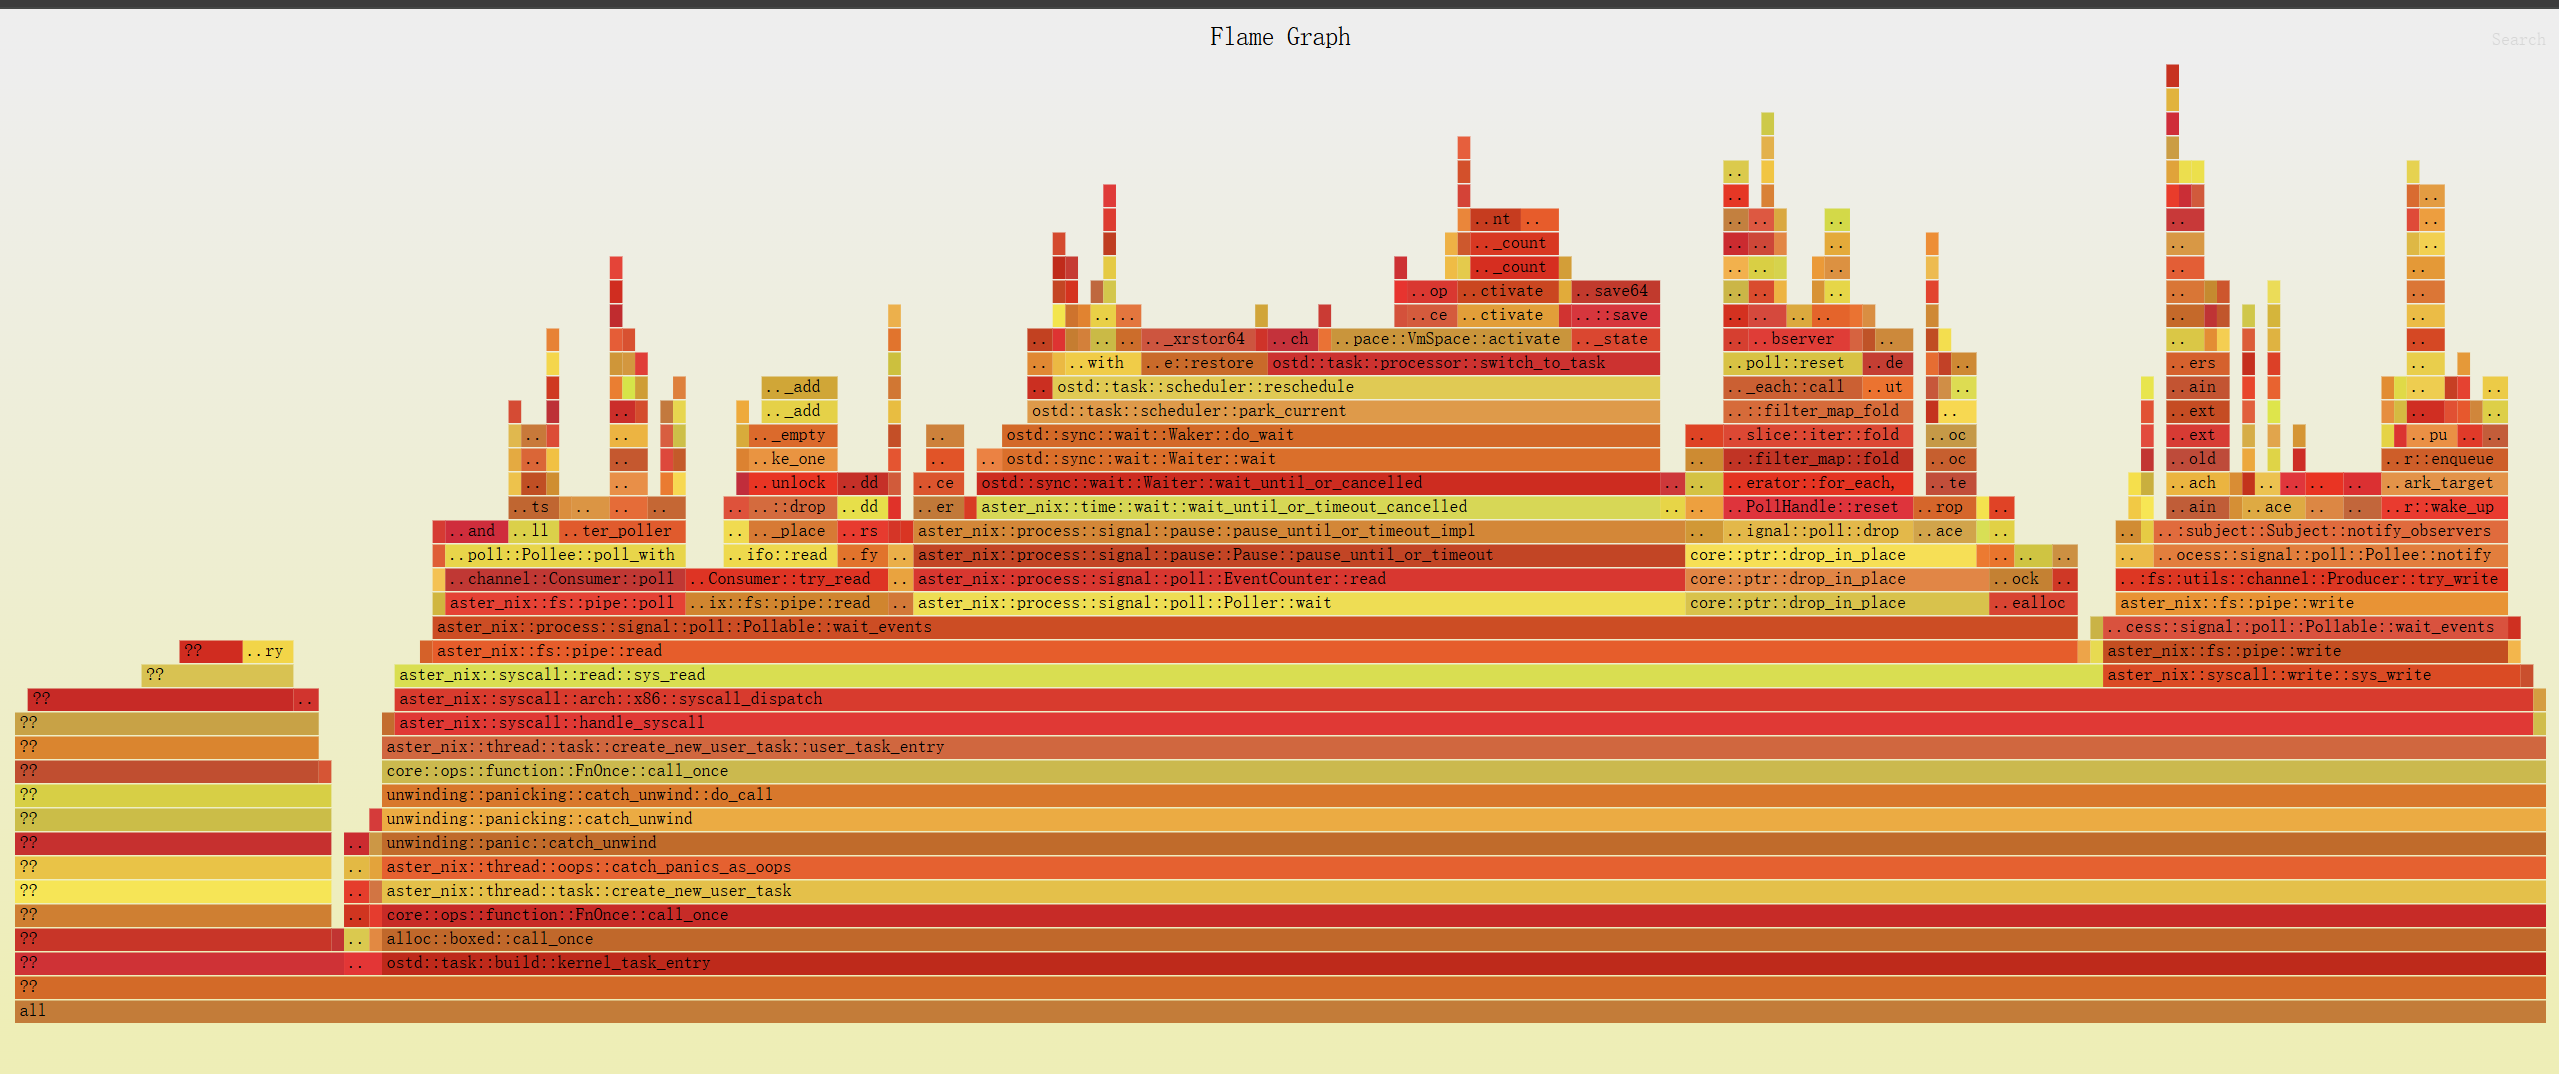
\includegraphics[width=\textwidth]{figure/before.png}
	\caption{Flame Graph of \texttt{lat\_pipe}}
\end{figure}

I choose to add time-consuming logics to the \texttt{inc\_ref\_count} function to slow down the process. The code modification and resulting flame graph are shown below.

\begin{figure}[H]
	\centering
	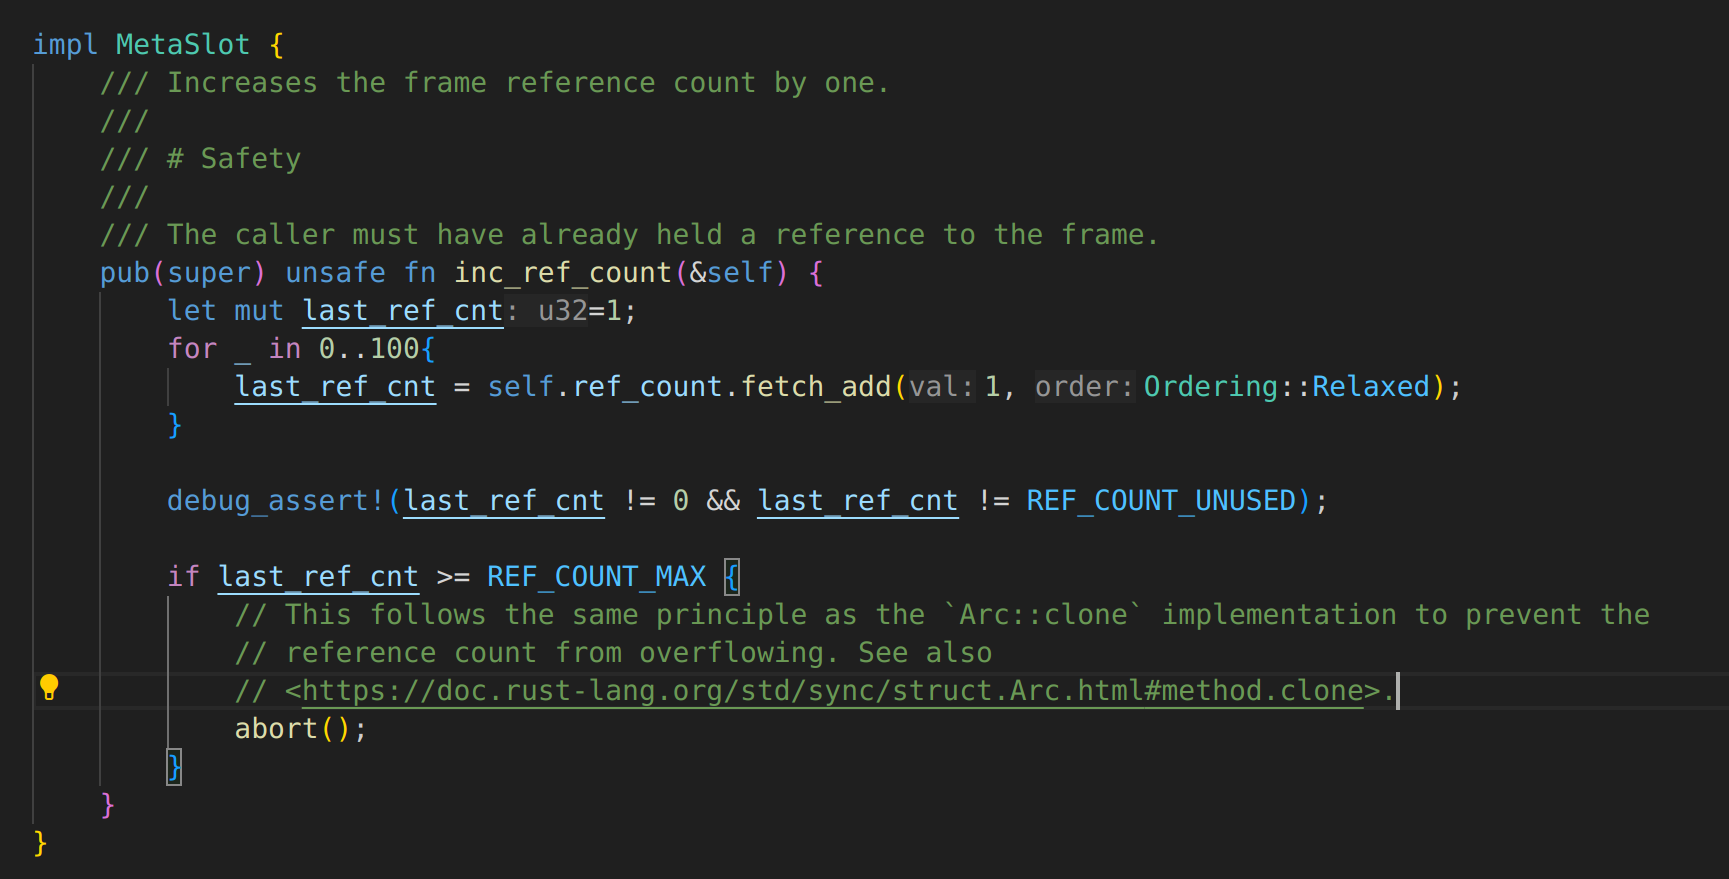
\includegraphics[width=0.8\textwidth]{figure/code.png}
	\caption{Code Modification}
\end{figure}

\begin{figure}[H]
	\centering
	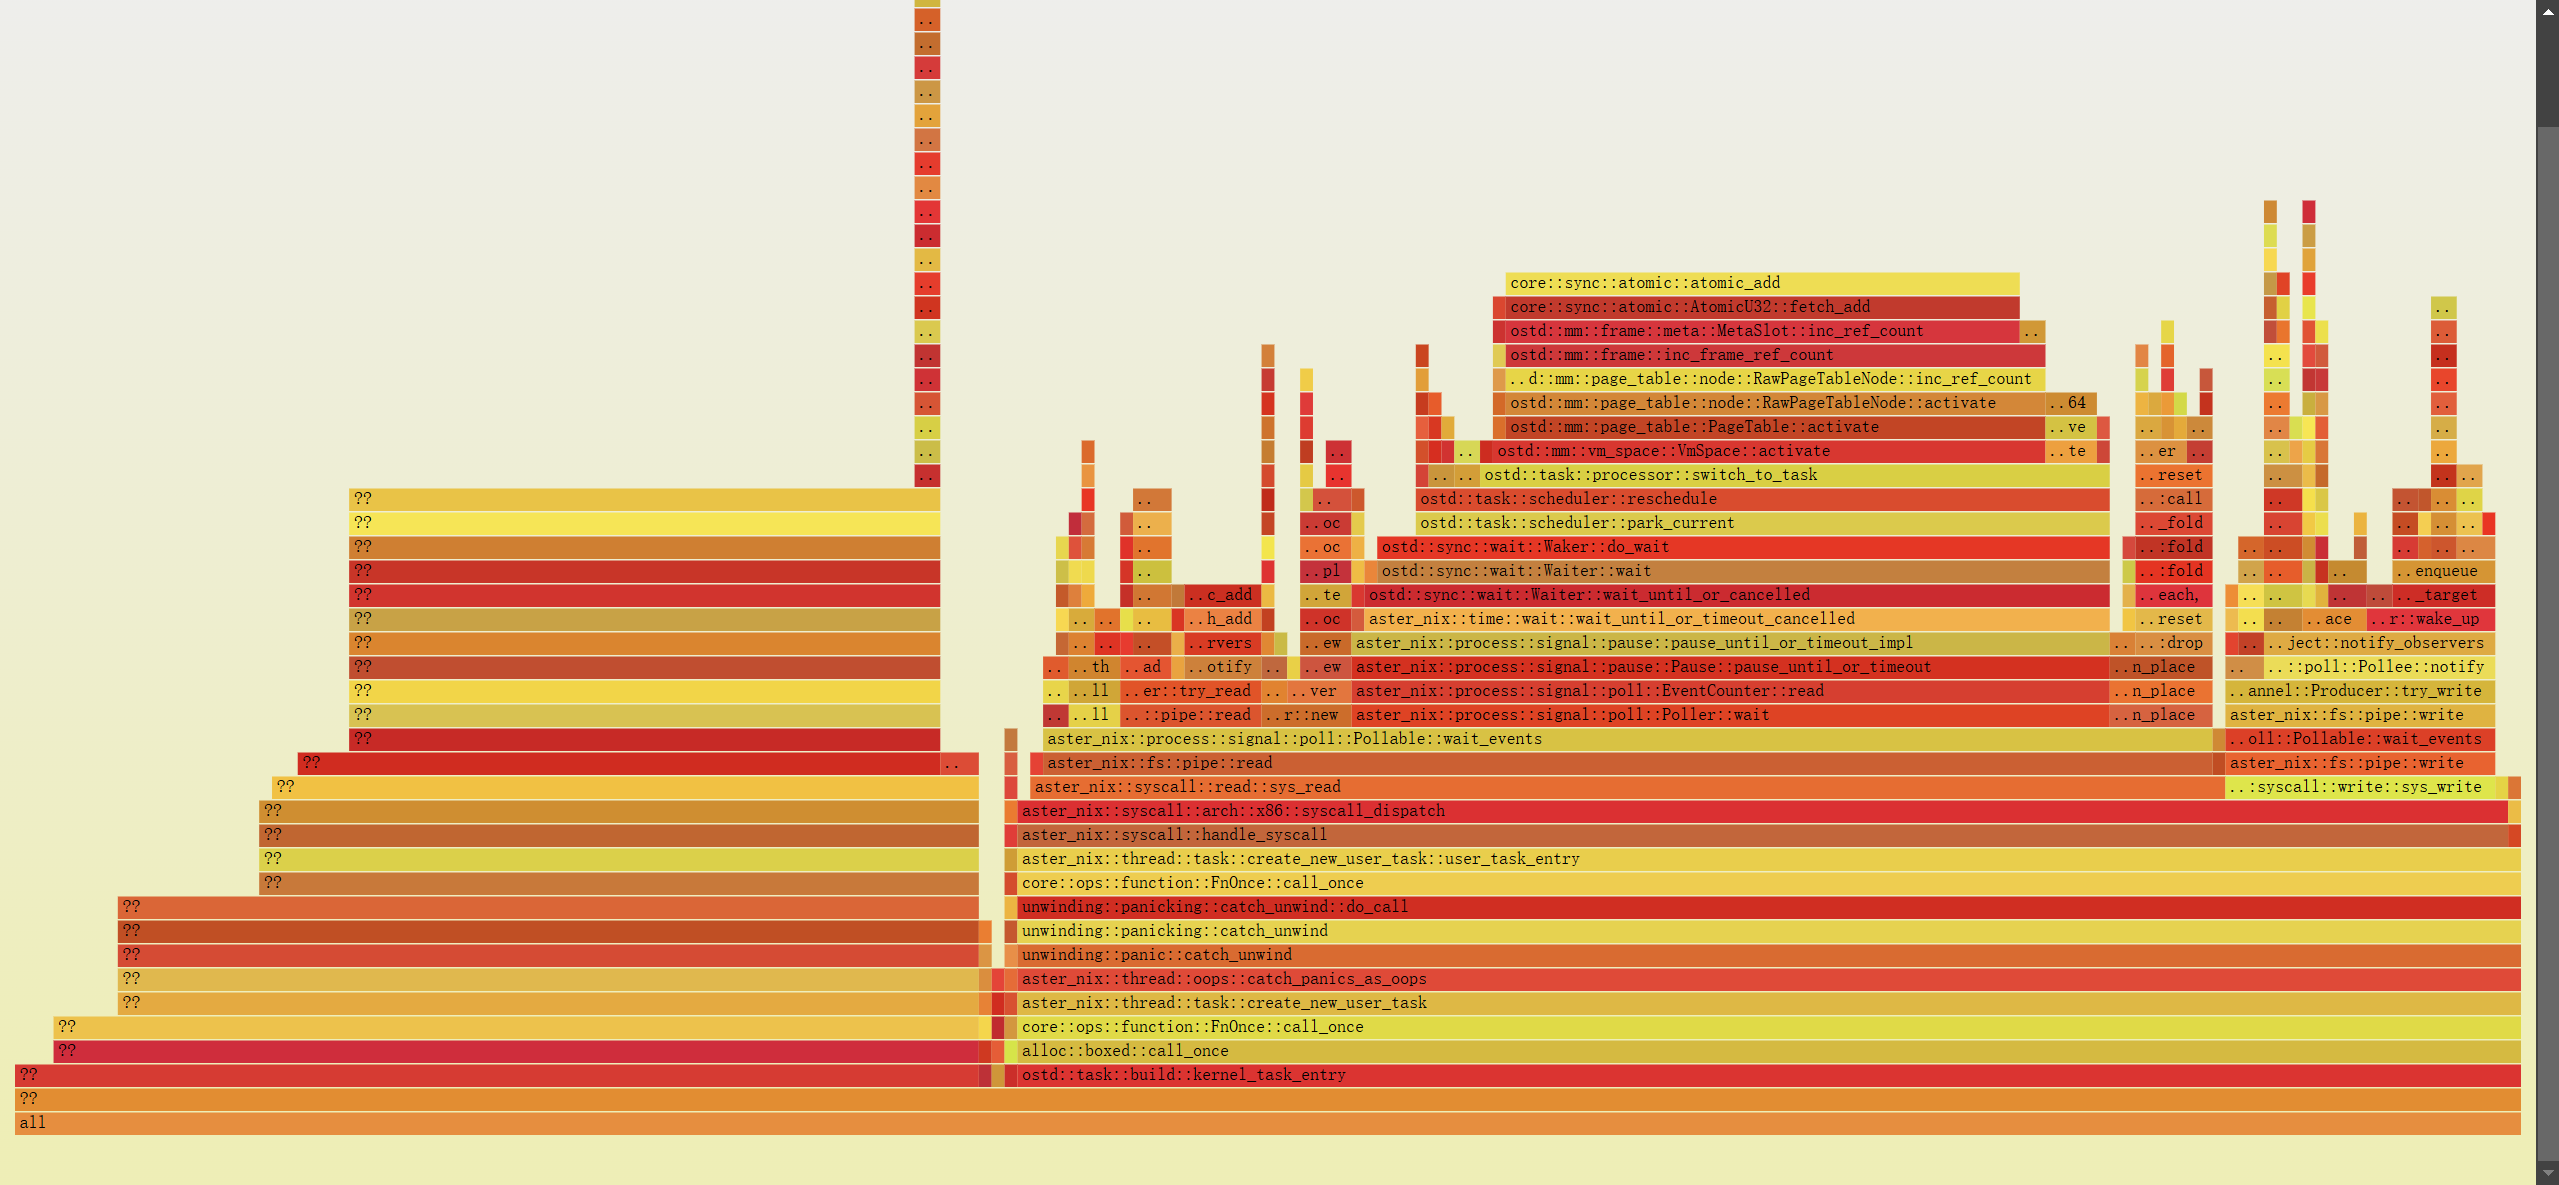
\includegraphics[width=\textwidth]{figure/after.png}
	\caption{Flame Graph of \texttt{lat\_pipe} after modification}
\end{figure}

It is obvious that the \texttt{inc\_ref\_count} function's time consumption is increased after the modification. 

\end{document}